\chapter{Preliminary Results}
\section{A trait-based characterization of phytoplankton communities in contrasting regions of the Atlantic Ocean}

\small {\textbf{Manuscript in preparation to be submitted to Marine Ecology Progress Series}}


\subsection*{}
\textbf{ABSTRACT}: In recent years trait-based ecology studies had been providing new insights on the mechanisms driving natural variation based on measurable key characteristics of organisms. Here we investigate the phytoplankton community size-composition in the Atlantic Ocean using data from the Atlantic Meridional Transect program. We extended the existing knowledge on the distribution of the phytoplankton size composition in the Atlantic, using a larger data set, integrating phytoplankton size composition, nutrients concentrations, and grazers abundance into a trait-based approach. The selected subset was constrain by k-means partitioning and based on the prevailing environmental conditions. Also we studied how the different phytoplankton size fractions respond to different environmental gradients. Our results suggest a linkage of the \textit{in situ} environmental conditions with community size-composition, and regardless of the spatio-temporal conditions. We discuss how the observed patterns of phytoplankton size-fractions in the Atlantic Ocean are coherent with the niche partitioning theory and opposed to the unified neutral theory of biodiversity.

\normalsize
\subsection{Introduction}
For many decades ecologist had been trying to understand how the recurrent patterns of community structure are associated to the environmental conditions, in particular, trying to understand the causes and consequences of natural variation. On the search for answers, ecologist had been measuring and testing their hypothesis based on observations of key characteristics of the organism, population or community. These key characteristics are nowadays referred as traits \citep{McGill2006, Violle2007}. 

Trait-based ecology attempt to develop general statements and predictability of natural communities, linking traits that influence the organism performances or fitness (i.e. functional trait) with the prevailing environmental conditions \citep{McGill2006}. For example, recent investigations suggest that mean trait variation and variance are invariable to different spatial scales, stressing the importance of the environment on trait variation and implying that the within-species and the interspecific variations on natural communities do not add more variation to the trait \citep{Messier2010}. The possibile understaning one could get implementing such an perspective into their research had motivated researchers to integrate more a trait-based perspective instead of the typical species-based approach to community ecology.

Phytoplankton communities are an ideal group of organisms to apply a trait-based approach. They are a well known group, with their ecological niche defined by the physical environment, the resource allocation strategy and the interspecific relationships \citep{Litchman2007}. They have various well understood morphological, physiological, behavioral and life history traits and trade-offs. Among all the known phytoplankton traits the cell-size is probably the best characterizing property of the phytoplankton communities \citep{Litchman2008,Litchman2010}. \textit{In vivo} and \textit{in situ} observations of a variety of traits are constantly measured due to the global importance of phytoplankton as primary producer, influencing trophic webs and biogeochemical cycles \citep{Falkowski1998}.

Almost every year, since 1995, two cruises have been take place crossing the Atlantic ocean from Plymouth, UK to South America or South Africa, measuring size fractionated chlorophyll-a, nutrient concentration (i.e. nitrate, phosphate, silicate), temperature and zooplankton abundance, among other parameters. These cruises belong to the Atlantic Meridional Transect Programme (www.amt-uk.org). This dataset is one of the most spatially extensive, allowing us to study the community composition and their driving processes at an ocean basin scale. Previuos investigations have been focussed on a description of the occurrences of the different size fractions \citep{Maranon2001} without a direct linkages to the prevailing environmental conditions. To our knowledge no efforts had been made to integrate and analyze the phytoplankton community size-structure using all available AMT dataset, and to link the mechanisms that shape the phytoplankton communities with the environmental conditions, regardless of the spatio-temporal scale.

Here we proposed a trait-based approach to study the response of the phytoplankton community size-structure to the environmental conditions at an ocean basin scale. We attempt to extent the existing knowledge of the phytoplankton communities on the Atlantic ocean, using a larger selection of data, and integrating phytoplankton size composition with temperature, nutrient concentrations, and grazers abundance into a trait-based perspective. To answer our research question first we used a known classification based on the environental conditions \citep{Longhurst2006} to constrain the data and related to phytoplankton community-size composition. Second we proposed a second classification using \textit{in situ} environmental conditions, and compared both methods. Third we related the environmental gradients to the community size-structure to study the emergent community patterns at ocean basin scale, and without any temporal constrian.

\subsection{Methods}

We used data provided by the Atlantic Meridional Transect (AMT) Program (www.amt-uk.org). We selected samples located in the mixed layer, with the parameters: size fractionated chlorophyll-a, nutrient concentration (i.e. Nitrate, Phosphate, Silicate), temperature and zooplankton abundance. The definition of mixed layer depth used was the depth at we can account variation in temperature of 0.5 $^\circ$C and in density of 0.125, fromthe first value at 5-10 dbar depth. We worked with a subset of 410 samples with information from 9 AMT cruises (AMT2, AMT3, AMT4, AMT5, AMT6, AMT10, AMT11, AMT13, AMT14). This cruises took place in April-May or September-October in the years, 1996 (AMT2 and AMT3), 1997 (AMT4 and AMT5), 1998 (AMT6), 2000 (AMT10 -AMT11) and 2003 (AMT13 and AMT14). 

\begin{wrapfigure}{r}{0.5\textwidth}
\begin{center}
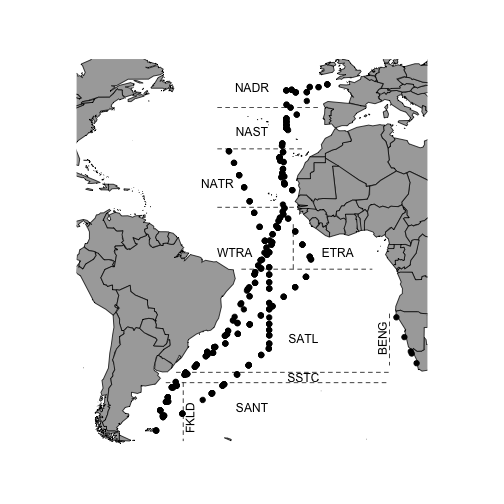
\includegraphics[trim = 30mm 15mm 25mm 15mm, clip, width=1\linewidth]{./Chp2-Pre/amt_mapFINAL2.png}
\end{center}
\caption[Scheme]{\small {AMT subset of 410 samples used on this study. The dashed lines represent the simplified limits of the Longhurst ecological provinces.}}
\label{Map}
\end{wrapfigure}

The phytoplankton size fractions considered were picoplankton (0.2-2 $\mu$m), nanoplankton (2 -20 $\mu$m) and microplankon ($>$20 $\mu$m). For the AMT13 and AMT14 cruises four size classes were measured (0.2-2, 2-5 5-10, $>$10 $\mu$m). Thus, to be consistent with the selected three size fractions we considered the 2-5 and 5-10 $\mu$m size classes as part of the nanoplankton class and the $>$10 $\mu$m class as part of the microplankton class. We checked for the results with and without these data and there was no difference in the observed patterns. The three size fractions were normalized, based on the proportion of each size fraction to the total chl-a concentration resulting in a range from 0 to 1.

The used subset cover temperate, subtropical and tropical regions of the Atlantic ocean (Figure \ref{Map}). According to \citet{Longhurst2006} ten ecological provinces were sampled by these cruises. They were four temperate provinces, the North Atlantic Drift (NADR; n=24), the South Subtropical Convergence (SSTC, n=21), Subantartic Water Ring (SANT, n=14) and the Falkland Island (FKLD; n=52); two subtropical provinces, the North Atlantic Subtropical Gyral (NAST; n=37) and the South Atlantic Subtropical Gyral (SATL, n=129); three tropical provinces, the North Atlantic Tropical Gyral (NATR, n=51), the Eastern Tropical Atlantic (ETRA, n=13) and the Western Tropical Atlantic (WTRA, n=64); and last, one upwelling region, the Benguela province (BENG, n=5). With this subset we analyzed the community size composition and implemented a linear mixed effect model (LME) to test if the community size-structure differs among ecological provinces. The ecological provinces were classified by regions, defined as: temperate (NADR, FKLD, SSTC, SANT), tropical (NATR, WTRA, ETRA), subtropical (SATL, NAST) and upwelling (BENG). The model was fitted to the data using each size fraction and the regions as fixed factors, and the ecological provinces as random factors.

We utilized a cluster analysis based on k-means partitioning to alternatively classified the data according to the prevailing environmental conditions. The environmental variables considered were nitrate + nitrite concentration, phosphate concentration, silicate concentration and temperature. A principal component analysis (PCA) of the environmental variables and the normalized size fractions was done to measure the relative importance of a specific environmental gradient to the phytoplankton size fractions. We quantified the linear relationships between the environmental and the community size-structure. In addition we also quantified the response of the three size fractions to the grazer abundance, but only using data of the cruises AMT3 and AMT5, due to a limited availability of the zooplankton abundance data on the rest of the cruises. The analysis was implemented in R v2.12.2 (The R Foundation for Statistical Computing, 2011).

\subsection{Results}

\begin{figure}
\centering
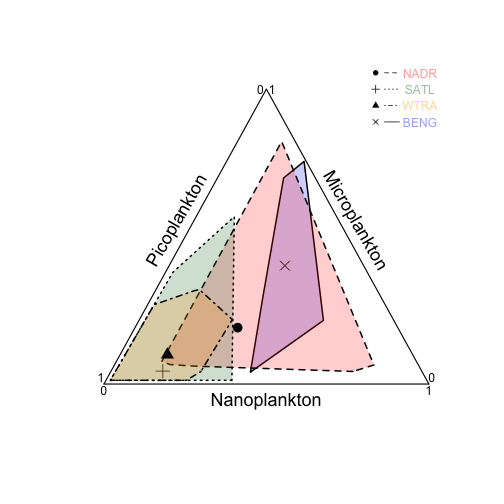
\includegraphics[trim = 15mm 15mm 15mm 15mm, clip, width=0.5\linewidth]{./Chp2-Pre/amt_4RegionsTriSizeFrac4.png}
\caption[Scheme]{\small {Phytoplankton community size structure of four ecological provinces in the Atlantic Ocean.The contours correspond to the convex hull of the size-fractions distribution on each province and the symbols denotes the mean values.}}
\label{RegSizeFrac}
\end{figure}

\begin{figure}
\centering
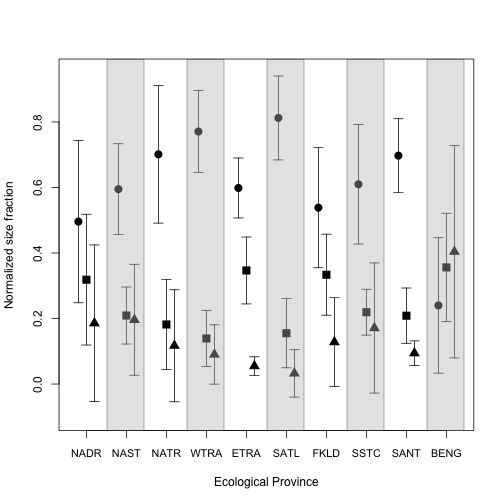
\includegraphics[trim = 0mm 0mm 0mm 0mm, clip, width=0.5\linewidth]{./Chp2-Pre/amt_MeanSDProvinces.png}
\caption[Scheme]{\small {Mean values ($\pm$sd) of three phytoplankton size fraction at ten ecological provinces of the Atlantic ocean. The symbols represent the mean of the picoplankton (\ding{108}), nanoplankton(\ding{110}) and microplankton (\ding{115}) normalized size fraction.}}
\label{means}
\end{figure}

Community size-structure is highly variable in different ecological provinces. (Figure \ref{RegSizeFrac}). Comparing the mean values of four selected provinces a increasing trend could be observed from the warmer provinces in the tropics and subtropics towards the colder provinces in the Benguela upwelling. Provinces in tropical and subtropical waters such as WTRA and SATL, showed a limited distribution of majorly picoplankton with some samples with data on nano- and microplankton. Temperate provinces such as NADR presented a spread distribution of size fractions in which the three size-fractions could dominate in the sample. The only upwelling province sampled showed a distribution of size fractions dominated more by nano- and microplankton. Thus, provinces located in temperate regions had a larger variability compared with provinces located in tropical regions (Figure \ref{means}). We found that these difference is significant for the picoplankton (LME/anova, df=3, F=6.6315, p=0.0247) and microplankton size fractions (LME/anova, df=3, F=5.5189,p=0.0368) but not for the nanoplankton size fraction (LME/anova, df=3, F=2.03341, p=0.2108).

\begin{figure}
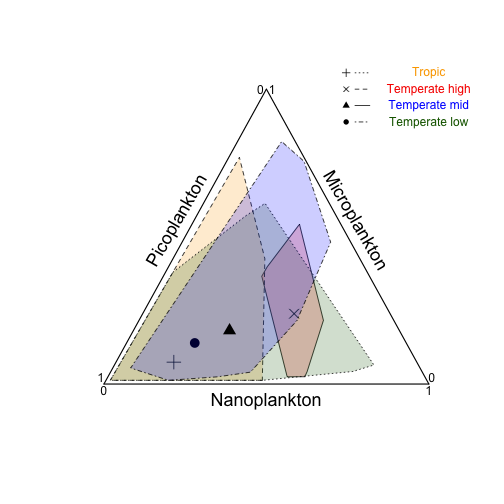
\includegraphics[trim = 12mm 10mm 10mm 15mm, clip, width=0.5\linewidth]{./Chp2-Pre/amt_clsEnvFINAL4.png}
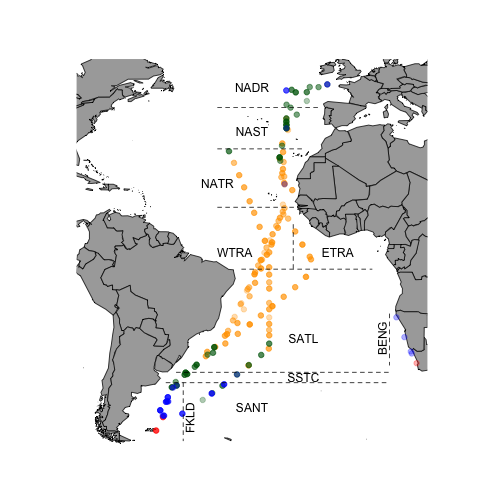
\includegraphics[trim = 20mm 10mm 20mm 10mm, clip, width=0.5\linewidth]{./Chp2-Pre/amt_mapClsEnv3.png}
\caption[Scheme]{\small {Phytoplankton community size structure based on the \textit{in situ} environmental conditions. Left: Distributions of size-classes in four clusters named: Tropic and Temperate with low, intermediate and high nutrient concentration. The contours correspond to the convex hull of the size-fractions distribution on each cluster and the symbols denotes the mean values.  Right: geographical distribution of the clusters compared with Longhurst classification. The color coding is according to the cluster classification.}}
\label{clusters}
\end{figure}

\begin{table}
\centering
\caption[Scheme]{\small {Mean values of in-situ environmental data by each cluster named: Tropic and Temperate with low, intermediate and hig nutrient concentration.}}
\label{tableclus}
\begin{tabular} {c c c c c}
cluster & $NO_3$ & $PO_4$ & $SiO_4$ & Temperature \\ \hline
Tropic & 0.150$\pm$0.575 & 0.064$\pm$0.078 & 1.097$\pm$0.575 & 25.299$\pm$2.000 \\
Temperate / Low N & 0.556$\pm$1.102 & 0.112$\pm$0.141 & 0.816$\pm$0.617 & 17.894$\pm$2.191 \\
Temperate / Interm. N & 9.027$\pm$3.593 & 0.799$\pm$0.373 & 2.423$\pm$1.375 & 11.925$\pm$2.797 \\
Temperate / High N & 30.324$\pm$4.549 & 1.336$\pm$0.208 & 4.590$\pm$1.926 & 6.810$\pm$3.435 \\ \hline
\end{tabular}
\end{table}

Tropical and subtropical regions share similar environmental conditions and community size composition while temperate regions possess different environmental conditions and more variable community structure (Figure \ref{clusters}). We separated all data according to their environmental properties into four clusters explaining 87.3$\%$ of the variability. The clusters are named according to the mean temperature (Tropic and Temperate) and the mean nutrient concentration (Temperate with low, intermediate and high nutrient concentration). The mean phytoplankton size composition of the clusters showed a increasing trend from the high-temperature low-nutrient regions (Tropics and Subtropics) towards the low-temperature high-nutrient regions (Temperate and Upwelling). Of the four environmental gradients temperature and nitrate+nitrite concentration are the most important variables explaining the variability of the data (Figure \ref{PrinComp}). The picoplankton size fraction is associated with temperature while the nutrient concentrations are associated with the nano- and microplankton size fractions.

The phytoplankton size composition varies with the environmental conditions, and without any temporal constrain (Figure \ref{response} and table \ref{stats}). An increase in nutrient concentration ($NO_3$, $PO_4$, $SiO_4$) led to a shift from picoplankton dominated community towards the nano- and microplankton dominated community. The same pattern was observed with the increase in the abundance of grazers (i.e. Copepods) where the picoplankton reduces from 70$\%$ to less than 40$\%$ and larger size-fractions such as the nanoplankton triplicates his abundace from 20$\%$ to 60$\%$. This last observation was only possible to make for two AMT cruises, for which we had a complete record of zooplankton abundance (AMT3 and AMT5). The size fraction response with temperature is inversed to the ones observed by the other environmental variables ($NO_3$, $PO_4$, $SiO_4$); where the picoplankton abundances duplicates with an increase of temperature, while the nano- and microplankton reduced to almost a half with an increase of temperature.


\begin{figure}
\centering
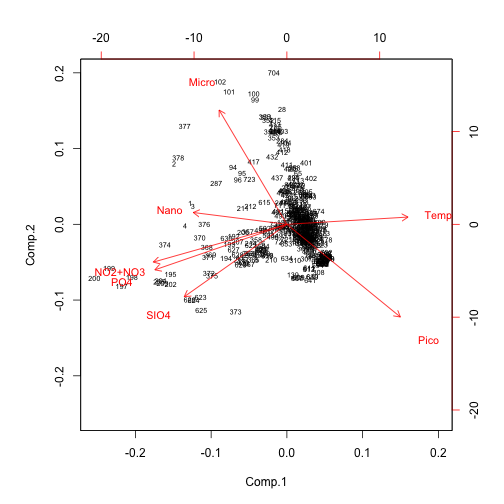
\includegraphics[trim = 0mm 0mm 0mm 0mm, clip, width=0.6\linewidth]{./Chp2-Pre/amt_PrinComp.png}
\caption[Scheme]{\small {Principal component analysis of environmental conditions and normalized phytoplankton size fractions.}}
\label{PrinComp}
\end{figure}

\begin{figure}
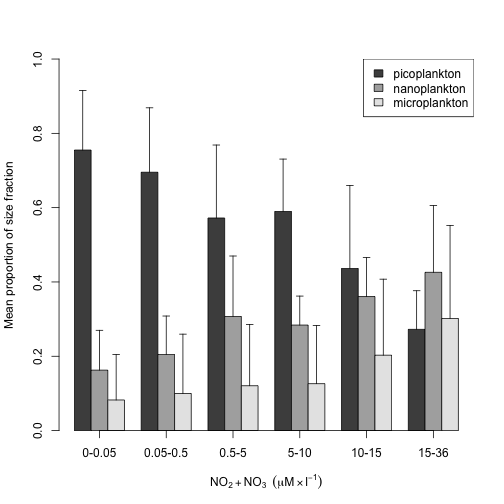
\includegraphics[trim = 0mm 0mm 0mm 15mm, clip, width=0.5\linewidth]{./Chp2-Pre/amt_NO3_bars2.png}
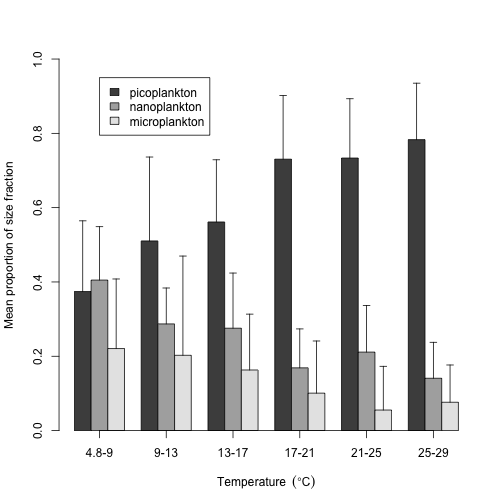
\includegraphics[trim = 0mm 0mm 0mm 15mm, clip, width=0.5\linewidth]{./Chp2-Pre/amt_Temp_bars2.png}
\includegraphics[trim = 0mm 0mm 0mm 15mm, clip, width=0.5\linewidth]{./Chp2-Pre/amt_zoo_bars2.png}
\caption[Scheme]{\small {Response of Picoplankton, nanoplankton and microplankton size fraction to Nitrate, Temperature and Zooplankton abundance. Bars represent mean values and the error bars the standard deviation.}}
\label{response}
\end{figure}

\begin{table}
\centering
\caption[Scheme]{\small {Summary statistics of linear fitting for the response of three size fractions to each environmental variable}}
\label{stats}
\begin{tabular} {c c c c c c c c c c }
& \multicolumn{3} {c} {Picoplankton} & \multicolumn{3} {c} {Nanoplankton} & \multicolumn{3} {c} {Microplankton} \\
& slope & p-value & $r^2$ & slope & p-value & $r^2$ & slope & p-value & $r^2$ \\ \hline
$NO_2+NO_3$ &-0.090 &0.002 & 0.908 &0.050 &0.001 & 0.921 &0.040 &0.010 &0.792 \\
$PO_4$ &-0.0812 &0.021 &0.711 &0.042 &0.012 &0.777 &0.039 &0.125 &0.354 \\
$SiO_4$ &-0.047 &0.085 &0.455 &0.030 &0.044 &0.597 &0.016 &0.247 &0.142 \\ 
Temperature &0.082 &0.001 &0.914 &-0.047 &0.008 &0.812 &-0.035 &0.003 &0.885 \\
Copepods &-0.063 &0.064 &0.520 &0.068 &0.051 &0.567 &-0.004 &0.788 &-0.222\\ \hline
\end{tabular}
\end{table}


\subsection{Discussion}
Using a single trait to characterize the phytoplankton community  we observed typical structural patterns on these communities, at an ocean basin scale and without any temporal constrain. In our trait based approach, we combine data of mainly two seasons (late spring/early summer and autumn) with almost a 10 year timespan and from different areas of the Atlantic Ocean and found, consistent patterns of phytoplankton size composition, such as, the dominance of picoplankton at oligotrophic waters (SATL) and at the tropics while at highly rich waters the larger size classes dominates (BENG) \citep{Maranon2000,Maranon2001,Poulton2006,Moreno-Ostos2011,Huete-Ortega2011}. We could observe that these patterns on the phytoplankton communities are strongly associate with the \textit{in situ} environmental conditions. For us these are very interesting results, considering the imposed preconditions in our analysis (Large spatial scale, no temporal constrain) what suggest that the propertives driving the structure of phytoplankton communitives are conservative.

The limited variation of size-fractions at tropical and subtropical regions compared to regions at temperate or upwelling areas, suggest that even due the environmental conditions at a regional scale are less variable (Tropics vs Temperate) yet the trait variation on some of those regions  (i.e. Temperate) is larger. This result is coherent with observations made by \citet{Messier2010} on trait variation of vascular plants. Where they argue that the environmental conditions strongly influence the trait distribution, but due to the high variability of the trait even regions with similar environmental conditions have a large trait variation. 

Comparing both classification methods, the Longhurst ecological regions make a clearer differense among the size-structures between the ecological provinces. However, the increased trend of the mean values is a shared propertive of both methods. Could be argue that the clearer differentiation with Longhurst is due to the historical characteristic of the environmental data he used build up his classification, while in our clustering approach we used actual environmental conditions that derive the observed community patterns.

Our clustering of the data by the \textit{in situ} environmental conditions suggest that the areas sampled between 30$^\circ$ N and 30$^\circ$ S consist of related nutrient and temperature conditions with a picooplankton dominated community. While the area in the extremes of those limits (Temperate regions), consist of colder waters with more nutrients and a wider range of phytoplankton size class. It is known that stronger seasonal shifts in temperate areas could lead shifts on the community composition. However, a temporal reconstruction from this dataset is not feasible due to the lack of temporal representative during a year. Nevertheless, these results are consistent with the observations made by previous studies on this dataset by \citep{Maranon2000, Maranon2001, Poulton2006} and by other observations in the tropical Atlantic\citep{Moreno-Ostos2011}. These authors suggest that nutrient uptake and light absorption traits are determinants for the size class distribution of phytoplankton in the Atlantic. But what we can observe is that not only nutrients and light but also temperature is one of the most influential environmental forcing. 

From the relationships analysed between the community size-structure and the environmental conditions NO$_3$, and temperature show a strong response for the different size fractions. While for PO$_4$, SiO$_4$ and the copepod abundance the response is significant only for the pico and nanoplankton size fractions. The size fractions could double or even triplicate their relative abundance under certain environmental gradients. This strong changes are explain by the trade-offs between cell-size with the energy and resourse utilization and the predation. Small phytoplankton have a competitive advantages over larger phytoplankton specially under low nutrient, low light and low grazing pressure conditions \citep{Litchman2008,Litchman2010}. And there are well known trade-offs between cell-size and: the nutrient acquisition, light absorption, sinking rates, abundance and grazing \citep{Kiorboe1993,Cermeno2008a,Finkel2009a}. Suppurting our results, that accordingly to the environmental conditions specific community structures will be observe. This is another interesting result, because, even this type of trends are already known, to our knowledge never have been observed, for a whole ocean basin and without any temporal constrain. 

In summary our trait-based approach to phytoplankton community composition in the Atlantic Ocean shows some interesting results. One of the most remarkable features of this analysis is how observing the variation of a key trait at ocean basin scale, and without any temporal limitation, still clear patterns of phytoplankton community structure could be tracked. Also these findings are consistent with Baas Becking tenet \citep{BaasBecking1934, DeWit2006,O'Malley2007}, demonstrating a relationship of the phytoplankton size fractions to large-scale environmental gradients, which also adds an interesting example to the discussion of niche vs. neutral theories \citep{Hubbell2001,Mcgill2003}. However, the hypothesis that the prevailing environmental conditions are major forces driving the phytoplankton communities in the Atlantic ocean should be study further. Future research should be focus on the mechanistic description of this dynamics similar to \citet{Falkowski2007} and using a trait-based modelling approach similar to \citet{Bruggeman2007, Merico2009} as suggested by \citet{Follows2011}. Such an approach will setup a theoretical framework to explore in detail the dynamics between the large-scale environmental influences on planktonic communities.

\subsection{Acknowledgements}
This study uses data from the Atlantic Meridional Transect Consortium (NER/0\\/5/2001/00680), provided by the British Oceanographic Data Centre and supported by the Natural Environment Research Council. 
